\section{Set Theory}
\chapquote{``A set is a Many that allows itself to be thought of as a One."}{Georg Cantor}

In questa sezione vengono presentate principalmente definizioni che forniranno la base per la trattazione dei successivi capitoli.
\subsection{Teoria di Zermelo-Frankel}
\subsection{Famiglie di insiemi}
\subsubsection{(axiom) Power set}
Sia $X$ un insieme. Denotiamo con $\mathcal P(X)$ l'insieme delle parti di $X$, definito come segue:
$$\mathcal P(X)\coloneqq \{ Y : Y\subseteq X\}$$
L'esistenza del power set è uno degli assiomi della Teoria degli Insiemi di Zermelo-Fraenkel.
\begin{figure}[H] % [H] makes sure the figure is placed exactly here
    \centering
    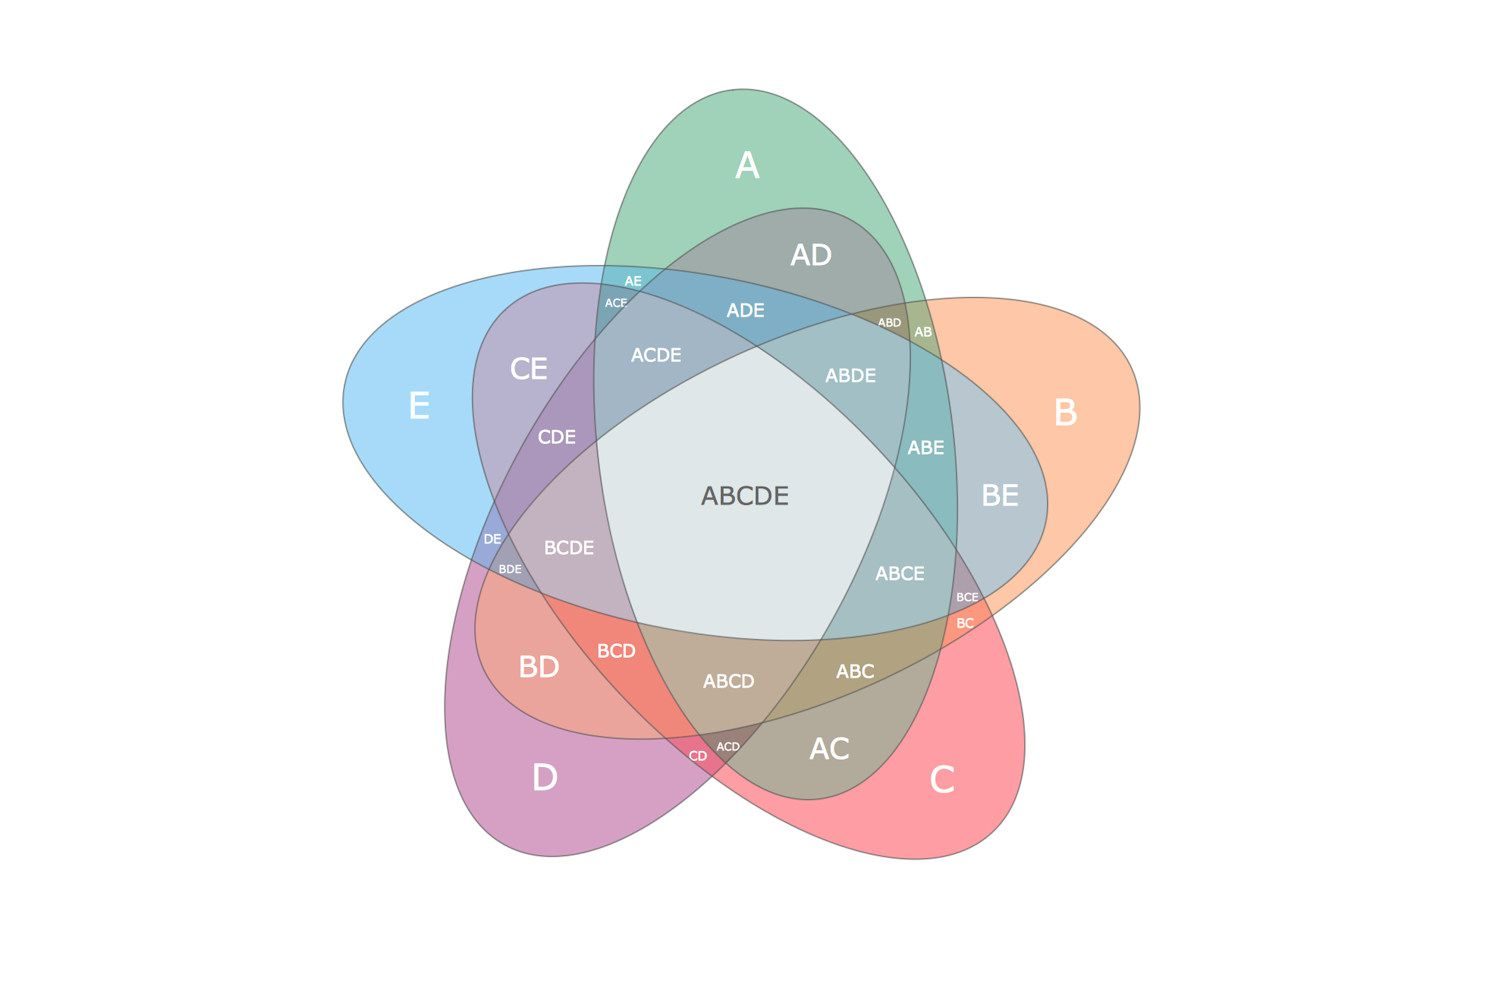
\includegraphics[width=0.7\textwidth]{assets/sets-5b180229ff1b780036cfb499.jpg}
    \caption{Insieme delle parti}
    \label{fig:example_image}
\end{figure}
Denotiamo con $\{E_i\}_{i\in I}$ una famiglia di insiemi indicizzata da I.\\

Una famiglia (o collezione) di sottoinsiemi di un insieme $X$ è $\{E_i\}_{i\in I}\subseteq \mathcal P(X)$
\subsubsection{(def) Union of a family of subsets}
Given a family $\{E_i\}_{i\in I}\subseteq \mathcal P(X)$,
$$\bigcup_{i\in I} E_i = \{x\in X\ : \ x\in E_i \text{ for some } i\in I\}$$
\subsubsection{(def) Intersection of a family of subsets}
Given a family $\{E_i\}_{i\in I}\subseteq \mathcal P(X)$,
$$\bigcap_{i\in I} E_i = \{x\in X\ : \ x\in E_i \text{ for every } i\in I\}$$
\subsubsection{(def) Pairwise disjoint family}
Una famiglia di insiemi $\{E_i\}_{i\in I}$ è detta disgiunta se
$$E_i\cap E_j=\emptyset \quad \forall i,j\in I:i\neq j$$
\subsubsection{(def) Convering set}
Una famiglia di insiemi $\{E_i\}_{i\in I}$ è detta copertura di $X$ se $$X\subseteq \bigcup_{i\in I}E_i$$
\subsubsection{(def) Subcovering}
Si definisce sottocopertura una sottofamiglia di una copertura di $X$ tale per cui essa stessa è ancora una copertura di $X$.
$$X\subseteq \bigcup_{i\in J}E_i\quad J\subset I$$
\subsection{Successioni di insiemi}
Le successioni (o sequenze) di insiemi sono un caso particolare di famiglia di insiemi in cui $I=\mathbb N$. Si denotano con $\{E_n\}_{n\in \mathbb N}$.
\subsubsection{(def) subsequence}
Una sottosequenza è una sequenza derivata da un'altra sequenza selezionando alcuni dei suoi elementi, mantenendo il loro ordine relativo.

Sia $\{E_n\}_{n\in \mathbb N}$ una sequenza. Una sottosequenza di $\{E_n\}_{n\in \mathbb N}$ è una sequenza della forma $\{E_{n_k}\}_{k\in \mathbb N}$
\subsubsection{(def) Monotone increasing (decreasing) sequence}
Una sequenza $ \{E_n\}_n\subseteq \mathcal P(X)$ è detta monotona crescente se:
$$E_{n}\subseteq E_{n+1} \quad \forall n \in \mathbb N$$

Analogamente, una sequenza $ \{E_n\}_n\subseteq \mathcal P(X)$ è detta monotona decrescente se:
$$E_{n}\supseteq E_{n+1} \quad \forall n \in \mathbb N$$


\subsubsection{(def) limsup e liminf di successioni di insiemi}
Considerando una sequenza $\{E_n\}_n\subseteq \mathcal P(X)$. Definiamo:
$$\limsup_n E_n = \bigcap_{k=1}^{+\infty}\Big [\bigcup_{n=k}^{+\infty} E_n\Big ]$$
$$\liminf_n E_n = \bigcup_{k=1}^{+\infty}\Big [\bigcap_{n=k}^{+\infty} E_n\Big ]$$
$$\limsup_n E_n=\liminf_n E_n=F \implies \lim_nE_n=F$$
\subsubsection{(def) Funzione caratteristica di un insieme}
Sia $E\subseteq X$, si definisce funzione caratteristica (o funzione indicatrice) la funzione $$\rchi_E(x)=\begin{cases}1\quad \text{se }x\in E\\0\quad\text{altrimenti}\end{cases}$$

\subsection{Relazioni}
Sia $X$ un insieme. Una relazione su $X$ è un sottoinsieme del prodotto cartesiano $R\subseteq X\times X$.
\subsubsection{(def) Relazione di equivalenza}
Una relazione $R$ si dice relazione di equivalenza e si indica con $\sim$ se soddisfa le seguenti proprietà:
\begin{enumerate}[label=\roman*]
    \item Riflessività $$(x,x)\in R\quad \forall x\in X$$
    \item Simmetria $$(x,y)\in R \iff (y,x)\in R$$
    \item Transitività $$\begin{cases}(x,y)\in R\\(y,z)\in R\end{cases}\implies (x,z)\in R$$
\end{enumerate}
Notazioni equivalenti: $(x,y)\in R \leftrightarrow xRy \leftrightarrow x\sim y$
\subsubsection{(def) classe di equivalenza}
Dato $a\in X$ e $\sim $ una relazione di equivalenza, definiamo:
$$[a]\coloneqq \{x\in X: x\sim a\}$$
la classe di equivalenza di $a$ su $X$.
\subsubsection{(prop) proprietà della classe di equivalenza}
\begin{enumerate}
    \item Ogni elemento di $X$ appartiene a una e una sola classe di equivalenza.
    \item Le classi di equivalenza formano una partizione di $X$, cioè suddividono $X$ in sottoinsiemi disgiunti, tali che la loro unione dà l'intero insieme $X$.
    $$X=\bigcup_{x\in X}[x]$$
\end{enumerate}
\subsubsection{(def) quotient set}
Il quotient set (insieme quoziente) è il risultato della "divisione" di un insieme $X$ in classi di equivalenza rispetto a una data relazione di equivalenza $\sim$.

L'insieme quoziente contiene quindi tutte le classi di equivalenza dell'insieme $X$ ed è una partizione di $X$.
$$\frac X R\coloneqq\{ [x]:x\in X\}$$
\subsubsection{(def) relazione d'ordine}
Una relazione d'ordine è una relazione binaria che stabilisce un confronto tra gli elementi di un insieme $X$, definendo un criterio di ordinamento.

Vi sono diversi tipi di relazioni d'ordine:
\begin{itemize}
    \item \textbf{Relazione di quasi ordine} se soddisfa le seguenti proprietà:
        \begin{enumerate}[label=\roman*]
            \item Riflessività $$xRx\quad \forall x\in X$$
            \item Transitività $$xRy , \ yRz\implies xRz$$
        \end{enumerate}
    \item \textbf{Relazione d'ordine parziale} se soddisfa le seguenti proprietà:
        \begin{enumerate}[label=\roman*]
            \item Riflessività $$xRx\quad \forall x\in X$$
            \item Antisimmetria $$xRy, yRx \implies x=y$$
            \item Transitività $$xRy , \ yRz\implies xRz$$
        \end{enumerate}
        Questo tipo di relazione permette di confrontare alcuni, ma non necessariamente tutti, gli elementi di $X$. Ci possono essere elementi non comparabili tra loro.
    \item \textbf{Relazione d'ordine totale (o lineare, o "catena")} se soddisfa le proprietà di un ordine parziale e si ha la connessione, ovvero $\forall a,b\in X$, vale o $aRb$ o $bRa$. Ovvero, ogni coppia di elementi è comparabile.
\end{itemize}
Ad esempio:
\begin{itemize}
    \item Ordine sui numeri reali: si sostituisca R con "$\le$". è un esempio di ordine totale.
    \item Sottoinsiemi di un insieme: si sostituisca R con "$\subseteq$". è un esempio di ordine parziale: es. $A=\{1\},\ B=\{2\}$, si vede che non vale l'ipotesi di connessione perché né $A\subseteq B$, nè $B\subseteq A$.
\end{itemize}

\subsection{Cardinalità degli insiemi}
\subsubsection{(def) Set equipotenti}
Dati due insiemi $X,Y$, questi si dicono equipotenti se esiste una bigezione $F:X\to Y$.
\subsubsection{(def) Cardinalità}
La cardinalità di $X$ è l'insieme di tutti gli insiemi equipotenti a $X$.
$$\vert X\vert \coloneqq \{ Y\  |\  \exists f:X\to Y \text{ bigettiva}\}$$
Ricorda che:
\begin{itemize}
    \item $f$ è iniettiva se $\forall x_1\neq x_2 \implies f(x_1)\neq f(x_2)$
    \item $f$ è suriettiva se per $f:X\to Y,\ Im(f)=Y$
    \item $f$ è bigettiva se è contemporaneamente iniettiva e suriettiva
\end{itemize}
\subsubsection{(def) Set finiti e infiniti}
Un insieme si dice:
\begin{itemize}
    \item infinito se esiste $E\subset X$ tale che $|X|=|E|$.
    \item Si dice finito se non è infinito.
\end{itemize}
\paragraph{Remark} If $X$ is finite, then it is equipotent to a set $\{1,2,\dots, k\}$ for an unique $k\in \mathbb N \ | \ k<+\infty$.
\subsubsection{(def) Set numerabile}
Un insieme $X$ si dice numerabile se $|X|\le |\mathbb N|$. Altrimenti sarà detto "non numerabile".

An infinite numerable set is said to have the $\aleph_0$ (aleph-zero) cardinality.
\paragraph{Which set is numerable?}\ \\
Of course $\mathbb N$ is numerable, it's easy to see that for every element of $\mathbb N$ corresponds the same element of $\mathbb N$. Let's consider other non-trivial examples:
\begin{itemize}
    \item $E=\{\text{even numbers of }\mathbb N\}$

    \begin{proof}
        We must prove that there exists a bijective function between $E$ and $\mathbb N$.
        We can consider the function
        $$f:\mathbb N\to E \quad\text{s.t. }f(n)=2n\quad \forall n\in \mathbb N$$
        \begin{itemize}
            \item Injection: \\
            We can prove that $f$ is injective by showing that $f(n_1)=f(n_2)\implies n_1=n_2$:
            $$f(n_1)=f(n_2)\implies 2n_1=2n_2\implies n_1=n_2$$
            \item Surjection:\\
            We can define $f^{-1}:E\to \mathbb N$ s.t. $f^{-1}(e)=\frac e2 \quad \forall e\in E$.

            To prove that $f$ is surjective, one can show that $f(f^{-1}(x))=x$. Applying the definition:
            $$f(f^{-1}(e))=2\frac e2 = e$$
            So every $e\in E$ has a preimage in $\mathbb N$.
        \end{itemize}
        Since $f$ is both injective and surjective, it is bijective.
    \end{proof}
    \item $\mathbb N^2$
    \begin{proof}
        \begin{itemize}
        We can start disposing all the couples $(a,b) \ : \ a,b\in \mathbb N^2$ in the following matrix:
        \begin{equation}
        \label{couples matrix}
        \begin{array}{cccccc}
        (0,0) & (0,1) & (0,2) & (0,3) & (0,4) & \dots \\
        (1,0) & (1,1) & (1,2) & (1,3) & (1,4) & \dots \\
        (2,0) & (2,1) & (2,2) & (2,3) & (2,4) & \dots \\
        (3,0) & (3,1) & (3,2) & (3,3) & (3,4) & \dots \\
        (4,0) & (4,1) & (4,2) & (4,3) & (4,4) & \dots \\
        \vdots & \vdots & \vdots & \vdots & \vdots & \ddots 
        \end{array}
        \end{equation}
        
        We can then enumerate all the couples starting from zero and proceding diagonally in this way:
        \begin{equation}
        \label{indeces matrix}
        \begin{array}{cccccc}
        0 & 2 & 5 & 9 & 14 & \dots \\
        1 & 4 & 8 & 13 & 19 & \dots \\
        3 & 7 & 12 & 18 & 25 & \dots \\
        6 & 11 & 17 & 24 & 32 & \dots \\
        10 & 16 & 23 & 31 & 40 & \dots \\
        \vdots & \vdots & \vdots & \vdots & \vdots & \ddots
        \end{array}
        \end{equation}
        We can now consider the \textit{Cantor's pairing function} that, for every couple $(a,b) \in \mathbb N^2$ in the matrix \ref{couples matrix}, returns its corresponding unique index ($\in \mathbb N$) from the matrix \ref{indeces matrix}:
        $$ \pi(a,b)=\frac{(a+b)(a+b+1)}{2}+b$$
        Thus, $\pi$ is a function that maps $\mathbb N^2$ into $\mathbb N$. It's inverse is given by:
        $$\begin{cases}
            a+b=w = \Big \lfloor \frac{\sqrt{8\pi+1}-1}{2}\Big\rfloor\\ b=\pi-\frac{w^2+w}{2}
        \end{cases}$$
        We can now start proving the bijection:
        \begin{itemize}
            \item Injectivity\\
            $$\pi(a_1,b_1)=\pi(a_2,b_2)\implies $$
            $$\frac{(a_1+b_1)(a_1+b_1+1)}{2}=\frac{(a_2+b_2)(a_2+b_2+1)}{2}+b_2$$
            Setting $w=a+b$,
            $$\frac{w_1(w_1+1)}{2}+b_1=\frac{w_2(w_2+1)}{2}+b_2$$
            $$\frac{w_1(w_1+1)}{2}-\frac{w_2(w_2+1)}{2}=b_2-b_1$$
            Suppose now that $w_1\neq w_2$.
            We know that $\frac{w_1(w_1+1)}{2}-\frac{w_2(w_2+1)}{2}$ is an integer different from $0$ because $w_1\neq w_2$.\\
            The difference $b_2-b_1$ is an integer that satisfies $|b_2-b_1|\leq |w_1-w_2|$ since $b\leq w$.
        \\
        Since the left term grows more rapidly than the right term, the inequality can be satisfied only if $w_1=w_2$, that also implies $b_2=b_1$ and so $a_1=a_2$
        \end{itemize}
                
        \end{itemize}
    \end{proof}
    \item $\mathbb Q$ (Rational numbers)
    \begin{proof}
        I'll first show the bijection between $\mathbb Q$ and $\mathbb N^2$, then the bijection between $\mathbb N^2$ and $\mathbb N$
    \end{proof}
\end{itemize}

\subsubsection{(thm) Cantor}
L'insieme delle parti di un insieme (il suo insieme potenza) ha sempre una cardinalità strettamente maggiore dell'insieme stesso.
$$|X|<|\mathcal P(X)|$$
Ad esempio, $\mathcal P(\mathbb N)$ ha la cardinalità del continuo.
\subsubsection{(conjecture) the continuum hypotesis}
L'ipotesi del continuo è una congettura formulata da Cantor. Essa afferma che non esiste un insieme la cui cardinalità sia strettamente compresa tra la cardinalità dei numeri naturali $\aleph_0$ e la cardinalità dei numeri reali $\mathfrak c$.
$$2^{\aleph_0}=\mathfrak c = \aleph_1$$
Nel 1940, Kurt Gödel dimostrò che l'ipotesi del continuo non può essere confutata all'interno della teoria degli insiemi di Zermelo-Fraenkel con assioma della scelta (ZF+AC), cioè è coerente con questa teoria assiomatica se essa stessa è coerente. Nel 1963, Paul Cohen dimostrò, utilizzando la tecnica del forcing, che l'ipotesi del continuo non può neanche essere dimostrata all'interno di ZF+AC. Questo significa che l'ipotesi del continuo è indipendente dagli assiomi della teoria degli insiemi: né può essere dimostrata né può essere confutata a partire da questi assiomi.
\subsubsection{(thm) Schröder-Bernstein}
$$\text{se }|X|\le |Y| \text{ e }|Y|\le |X|\implies |X|=|Y|$$
Questo teorema è utile, ad esempio, nel confronto tra insiemi infiniti, in quanto permette di stabilire che due insiemi hanno la stessa cardinalità senza dover costruire esplicitamente una biezione tra di loro.
\subsubsection{(axiom) Assioma della scelta}
Data una famiglia di insiemi non vuoti $\{X_i\}_{i\in I}$, esiste una funzione $f$ detta funzione di scelta tale che, per ogni insieme $X_k\in \{X_i\}_{i\in I}$, si ha che $f(X_k)\in X_k$.

In altre parole, per ogni collezione di insiemi non vuoti, si può scegliere un elemento da ciascuno di questi insiemi, anche senza specificare un criterio particolare di selezione.

\paragraph{Esempio semplice}
Immagina di avere un insieme infinito di scatole, ognuna contenente almeno un oggetto. L'assioma della scelta garantisce che è possibile selezionare un oggetto da ciascuna scatola, anche se non abbiamo una regola esplicita per decidere quale oggetto prendere da ogni scatola.

\paragraph{Equivalenze con altri teoremi}
L'assioma della scelta è equivalente (nel senso che se è vero l'assioma, sono veri anche questi teoremi, e viceversa) ai seguenti risultati:
\begin{itemize}
    \item Lemma di Zorn
    \item Teorema di Hausdorff: che garantisce che ogni insieme ben ordinato ha una cardinalità.
    \item Teorema di Tychonoff: che afferma che il prodotto arbitrario di spazi topologici compatti è compatto.
\end{itemize}
\paragraph{Relazione con la teoria ZF}
L'assioma della scelta non è dimostrabile all'interno della teoria degli insiemi standard di Zermelo-Fraenkel (ZF), quindi viene spesso aggiunto come un assioma supplementare, formando la teoria degli insiemi ZF+AC (Zermelo-Fraenkel con assioma della scelta). Questa versione estesa della teoria è nota come ZFC.
\subsubsection{(def) maximal element}
Sia $(S,\le)$ un insieme parzialmente ordinato. Un elemento $m\in S$ è detto elemento massimo se:
$$ \forall x\in S, \text{ se }m\le x, \text{ allora }m=x$$
\subsubsection{(def) upper bound}
Sia $A$ un insieme e $\le$una relazione d'ordine su un insieme $X\supset A$, allora un elemento $u\in X$ è detto upper bound di $A$ se:
$$\forall a \in  A,\ a\le u$$

Inoltre, se $u\le v, \forall v\ :\  v \text{ is an upperbound of }A\implies u=\sup(A)$, ovvero il minimo degli upperbounds di A.
\subsubsection{(lemma) Zorn's lemma}
Dato un insieme $P$ parzialmente ordinato, se ogni catena ha un upperbound, allora $P$ ha un elemento massimale.

